\section{Impact of radiation on electronics \& optoelectronics (\textbf{OAA~30pp})}
\label{sec:electronics}

{\it Editors: M. Bindi, E. Butz}  \\
{\it Contibuting authors: M.~Backhaus; M.~Bindi; P.~Butti; E.~Butz; W.~Erdmann; R.~Gerosa; B.~Haney; H.~Hillemanns; K.~Padeken; F.~Pinto; G.~Pownhall; D.~Robinson; A.~Rozanov, J.~Troska; T.~Weidberg.}  \\

\noindent 
In this chapter we will present the results of the impact of radiation on electronics and opto-electronics for the four LHC experiments during Run1 and Run2. ATLAS results are presented in section \ref{sec:electronics-ATLAS}; CMS in section  \ref{sec:electronics-CMS} whilst LHCb and ALICE observations are described in section  \ref{sec:electronics-ALICE-LHCb}. In section \ref{sec:electronics-comparisons} we will present the comparison between the various experiments; finally, in section \ref{sec:electronics-conclusions}, some guidelines and suggestions  for building and operating electronics and opto-electronics in future LHC experiments will be given.

\subsection{ATLAS}
\label{sec:electronics-ATLAS}
Contributing author: M. Bindi;
\noindent 

The ATLAS Inner Detector (ID) has been designed to provide hermetic and robust pattern recognition, 
excellent momentum resolution and both primary and secondary vertex measurements for charged tracks within the pseudorapidity range \mbox{$|\eta|<2.5$}.

The ID layout, described in \cite{jinst3s08003}, reflects the performance requirements: the ID is contained within a cylindrical
envelope of length $3512\,{\text{mm}}$ and of radius $1150\,{\text{mm}}$, within a solenoidal magnetic field of
$2\,{\text{T}}$. The ID consists of three independent but complementary sub-detectors: at inner radii, high-resolution pattern
recognition capabilities are available using discrete space-points from the silicon Pixel detector (\mbox{$r\leq122.5\,{\text{mm}}$}) and
stereo pairs of silicon microstrip from the Semiconductor Tracker (SCT)
(\mbox{$299\geq r\leq514\,{\text{mm}}$}); at larger radii (\mbox{$563\geq r\leq1066\,{\text{mm}}$}), the transition radiation
tracker (TRT) comprises several layers of gaseous straw tube elements interleaved with transition radiation material. 
 
The performance of the ATLAS experiment depends critically on the innermost layer (B-layer) of the Pixel detector. 
For this reason, at the beginning of 2013 the detector underwent the first of three long shutdown (LS) phases planned by the LHC machine. 
During this period (LS1), a fourth pixel layer based on new technology, the Insertable B-Layer (IBL)\cite{IBLPaper}, 
was added to the pixel detector between a new, narrower Beryllium beam-pipe and the pre-existing B-Layer. 

Fig.~\ref{fig:IDRun2Layout} shows the r-z layout of the upgraded ID during Run-2.

\begin{figure}
  \centering\includegraphics[width=1\linewidth]{figures/ElectronicsChapter/ATLAS/ID_Run2Layout.pdf}
  \caption{The r-z cross-section view of the layout of the ATLAS inner detector for Run 2. The top panel shows the
whole inner detector, whereas the bottom panel shows a magnified view of the Pixel detector region..}
  \label{fig:IDRun2Layout}
\end{figure}

At the same time, during LS1, pixel services were replaced by new ones (new Service Quarter Panel, or nSQP). 

After resuming data-taking in 2015, ATLAS has successfully operated the ID during
Run-2 at  \mbox{$\sqrt{s}=13\,{\text{TeV}}$} and instantaneous luminosities surpassing the design value of \mbox{$1\times10^{34}\,{\text{cm}}^{-2}{\text{s}}^{-1}$}.
The total integrated luminosity collected till 2019 by Pixel, SCT and TRT detectors is $\sim\,190 fb^{-1}$ whilst the IBL detector, operating only during Run 2, collected a luminosity of  $\sim\,159 fb^{-1}$.

Radiation effects from TID on the IBL front-end electronics will be described in section \ref{sec:electronics-ATLAS-TID}; SEU/SET effects from highly ionizing particles in IBL and SCT detector will be shown in section \ref{sec:electronics-ATLAS-SEU} whilst impact on opto-electronics from SCT will be described in section \ref{sec:electronics-ATLAS-Opto}. Finally, results from TRT electronics will be presented in section \ref{sec:electronics-ATLAS-TRT}

\subsubsection{TID effects in the IBL front-end chip (\textbf{4 pp})} 
\label{sec:electronics-ATLAS-TID}
Contributing authors: M.Backhaus; A.LaRosa;

%\subsubsubsection{Introduction}
\noindent 
The IBL consists of 14 carbon fibre staves instrumented along 64\,cm, 2\,cm wide, and tilted in $\phi$ by 14$^{o}$  surrounding the beam-pipe at a mean radius of 33\,mm  from the beam axis and providing a pseudo-rapidity coverage of $\pm$\,3. Each stave, with integrated CO$_{2}$ cooling, is equipped with 32 front-end chips bump bonded to silicon sensors.\\
The IBL detector was designed to be operational until the end of the LHC Run~3, where the total integrated luminosity was expected to reach $300~{\rm fb^{-1}}$. The detector components are qualified to work up to 250\,Mrad of total ionising dose (TID).\\
The IBL front-end chip,  namely FE-I4 ~\cite{FEI4},  was designed in 130\,nm CMOS technology which features an array of 80\,x\,336 pixels with a pixel size of 50\,x\,250\,$\mu$m$^{2}$. Each pixel contains an independent, free running amplification stage with adjustable shaping, followed by a discriminator with independently adjustable threshold. The FE-I4 keeps track of the time-over-threshold (ToT) of each discriminator with 4-bit resolution, in counts of an external supplied clock of 40\,MHz frequency.
The FE-I4 operates by feeding the common power supply to analog signal amplifiers and digital signal-process circuits, referred to as the low-voltage (LV) power supply and the clock input.\\
  
\subsubsubsection{Observations during 2015 data taking}
During the first year of the IBL operation in 2015, a significant increase of the LV current of the front-end chip and the detuning of its parameters (threshold and time-over-threshold) have been observed in relation to the received TID.

The LV current of the FE-I4 chip was stable at a value of 1.6--1.7\,A (for a four-chip unit) until the middle of September 2015.  Then, the current started to rise up significantly (see Figure~\ref{fig:IBL_LVdrift2015}), and the change of the current during September to November 2015 was more than 0.2\,A even within a single LHC fill, depending on the luminosity and the duration of the fill.

\begin{figure}[h!]
\centering
\includegraphics[width=3.5in]{figures/ElectronicsChapter/ATLAS/IBL_LVdrift2015.pdf}
\caption{Mean low voltage (LV) current in IBL FE-I4 chips during stable beam as a function of integrated luminosity and total ionising dose (TID). In the period from September to November 2015 the IBL detector was switched off during one LHC fill (due to safety concerns in early October 2015). The mean LV currents are averaged for all modules across 100 luminosity blocks and there is no obvious dependence of LV current on module group position. The TID is calculated from integrated luminosity~\cite{TaskForceNote}.}
\label{fig:IBL_LVdrift2015}
\end{figure}

With the increase of the LV current, the temperature of IBL modules also changes (Figure~\ref{fig:correlation_T_I_2015}).

\begin{figure}[h!]
\centering
\includegraphics[width=3.5in]{figures/ElectronicsChapter/ATLAS/correlation_T_I_2015.pdf}
\caption{Performance of the IBL modules during high luminosity proton-proton collision runs from September to November 2015, separated into the periods before (red circles) and after (black triangles) the long power-off on October 6. The data are displayed as a function of the average module current per 4 front-ends of the IBL and compared to a linear dependence. The average module temperature is shown~\cite{TaskForceNote}.}
\label{fig:correlation_T_I_2015}
\end{figure}
%
In addition, as shown for example in Figure~\ref{fig:IBL_ToTdrift}, the calibration of the FE-I4 chips for the analog discriminator threshold and the target ToT were observed to drift rapidly despite frequent updating of the calibration.
%
\begin{figure}[h!]
\centering
\includegraphics[width=3.5in]{figures/ElectronicsChapter/ATLAS/IBL_ToTdrift.pdf}
\caption{The time-over-threshold (ToT) and its RMS as a function of the integrated luminosity or total ionising dose (TID)~\cite{TaskForceNote}. The detector was regularly retuned, and each marker type corresponds to a single tuning of the detector.}
\label{fig:IBL_ToTdrift}
\end{figure}

The increase of the LV current  of the FE-I4 chip and the drifting of its tuning parameters were traced back to the generation of a leakage current in NMOS transistors induced by radiation higher than usual. The radiation induces positive charges that are quickly trapped into the shallow-trench-insolation (STI) oxide at the edge of the transistor. Their accumulation builds up an electric field sufficient to open a source-drain channel where the leakage current flows. If the accumulation of positive charges is relatively fast, the formation of interface states is a slower process. The negative charges trapped into interface states start to compete with the oxide-trapped charges with a delay. This is what gives origin to the so called rebound effect~\cite{FACCIO}. 

\subsubsubsection{Irradiation test-results}

Dedicated laboratory measurements~\cite{LAURA} of irradiated single transistors in 130\,nm CMOS commercial technologies showed that the increase of the leakage current reaches its peak value between 1\,Mrad and 3\,Mrad. For higher TID the current decreases to a value close to the pre-irradiated one. \\
To reproduce and analyse the effects described above during the FE-I4 chip operation, several  irradiations and electrical tests 
were performed~\cite{TaskForceNote}. Since the current increase in NMOS transistors depends on dose rate and temperature, measurements under different temperature and dose rate conditions have been carried out to qualify this dependency.\\
The first irradiation test aimed at measuring the boundary current (at a given temperature and dose rate) that the chip always approaches after annealing periods and re-irradiation. Figure~\ref{fig:ThreePeaks} shows the increase of the current consumption of a single FE-I4 chip in data taking condition as a function of the TID. The temperature of the chip was 38\,$^\circ$C and the dose rate 120\,krad\,h$^{-1}$. After reaching the maximum of each peak the chip was annealed for several hours resulting in the observed partial recovery. 
%
\begin{figure}[h!]
\centering
\includegraphics[width=3.5in]{figures/ElectronicsChapter/ATLAS/ThreePeaks.pdf}
\caption{Current consumption of a single FE-I4 chip in data taking condition as a function of the total ionising dose (TID). The temperature of the chip was 38\,$^\circ$C and the dose rate 120\,krad\,h$^{-1}$. After reaching the maximum of each peak the chip was annealed several hours resulting in the observed partial recovery~\cite{TaskForceNote}. The fit performed on the first set of data (first peak) has been carried out by using the current parametrisation described in Ref.~\cite{MALTE}.}
\label{fig:ThreePeaks}
\end{figure} 
%
Then, to study the dependence of the LV current increase on temperature and dose rate several irradiation tests were performed by setting one of those  variables and changing the other. 
Figure~\ref{fig:TemperatureComparison} shows the results of three different measurements, performed with 
three different and previously not irradiated chips. The dose rate was 120\,krad\,h$^{-1}$  and the temperatures were 38\,$^\circ$C, 
15\,$^\circ$C and $-$\,38\,$^\circ$C. Before irradiation the LV current of the three chips was 400\,mA (38\,$^\circ$C), 
360\,mA (15\,$^\circ$C) and 380\,mA ($-$\,38\,$^\circ$C).
For comparison Figure~\ref{fig:DoserateComparison} shows the result of two different measurements where the temperature was kept fix at 15\,$^\circ$C, while the dose rate  set to 120\,krad\,h$^{-1}$  or 420\,krad\,h$^{-1}$. Also in this case the tests were performed with different and previously not irradiated chips. 
%
\begin{figure}[h!]
\centering
\includegraphics[width=3.5in]{figures/ElectronicsChapter/ATLAS/TemperatureComparison.pdf}
\caption{Increase of the LV current of three single FE-I4 chips in data taking condition as a function of the total ionising dose (TID) 
in logarithmic x-axis scale. Test measurements were carried out at 38\,$^\circ$C (blue points), at 15\,$^\circ$C (black points) and at $-$\,15\,$^\circ$C (red points) with a dose rate of 120\,krad\,h$^{-1}$. A dose rate up to 10\,krad\,h$^{-1}$ is expected in the experiment. The LV current of the single FE-I4 chips before irradiation were 400\,mA (38\,$^\circ$C), 360\,mA (15\,$^\circ$C) and 380\,mA ($-$\,38\,$^\circ$C)~\cite{TaskForceNote}.}
\label{fig:TemperatureComparison}
\end{figure} 
%
\begin{figure}[h!]
\centering
\includegraphics[width=3.5in]{figures/ElectronicsChapter/ATLAS/DoserateComparison.pdf}
\caption{Increase of the LV current  of two single FE-I4 chips in data taking condition as a function of the total ionising dose (TID) in logarithmic x-axis scale. Test measurements were carried out at 15\,$^\circ$C with a dose rate of 120\,krad\,h$^{-1}$ (red points) and 420\,krad\,h$^{-1}$ (black points). A dose rate up to 10\,krad\,h$^{-1}$ is expected in the experiment. The LV current of the single FE-I4 chips before irradiation were 380\,mA (420\,krad\,h$^{-1}$) and 360\,mA (120\,krad\,h$^{-1}$)~\cite{TaskForceNote}.}
\label{fig:DoserateComparison}
\end{figure} 
%
The measurements described above revealed two facts: 
\begin{itemize} 
\item at a given dose rate the LV current increase is stronger at lower temperatures; 
\item at a given temperature, the LV current increase is stronger at higher dose rates.
\end{itemize}
To simulate the dose rate conditions of the 2015 and 2016 data taking, a first irradiation was performed at $-$15\,$^\circ$C and 120\,krad\,h$^{-1}$. This was followed by several hours of annealing and a second irradiation this time performed at 5\,$^\circ$C and 420\,krad\,h$^{-1}$.
As shown in Figure~\ref{fig:MixedIrradiaiton} the second LV current peak is lower than the first one, i.e. by increasing the operational temperature of the chip it was possible to keep the increase of the LV current below the boundary current given by the first irradiation. 
%
\begin{figure}[h!]
\centering
\includegraphics[width=3.5in]{figures/ElectronicsChapter/ATLAS/MixedIrradiaiton.pdf}
\caption{Increase of the LV current of a single FE-I4 chip in data taking condition as a function of the total ionising dose (TID) in logarithmic x-axis scale during two consecutive irradiation campaigns in a lab measurement. Between the two irradiations several hours of annealing period at room temperature was performed, and resulted in the observed recovery. The TID of both irradiations is summed up. The LV current of a single FE-I4 chip before irradiation was 380\,mA (first step) and 550\,mA (second step)~\cite{TaskForceNote}.}
\label{fig:MixedIrradiaiton}
\end{figure} 
%
To verify that a temperature of 5\,$^\circ$C is safe for the IBL detector operation, a measurement  at 10\,krad\,h$^{-1}$ was performed. The maximum LV current increase was of the order of 250\,mA, which gives a LV current increase of 1\,A for a four-chip unit, which would not exceed the safety limit of the LV current originally set to 2.8\,A.\\
In principle, lower operational temperatures are favourable for the sensor performance and properties after irradiation and therefore preferred. Consequently, irradiation and electrical tests were also performed at a temperature of 0\,$^\circ$C to investigate the feasibility for a colder operation.
In addition it was investigated the evolution of the maximum of the LV current peak under several irradiation steps followed, interleaved with periods of annealing.
In this case the first two consecutive peaks of the LV current increase exceeded the maximum current allowed for a safe detector operation. Therefore, it was decided to set 5\,$^\circ$C as minimum temperature for a safe and successful data taking.

\subsubsubsection{Detector operation guidelines}
Based on the observations during the first year of data-taking in 2015 with the IBL detector, it was decided to raise the safety limit for the IBL LV currents from 2.8\,A to 3\,A for module groups of four chips, which means a current consumption of 750\,${\mathrm{mA}}$ per chip. 
Since the average current consumption for a sigle FE-I4 chip  is about 400\,${\mathrm{mA}}$ before irradiation, the increase of the current due to the TID effects can not be higher than 350\,${\mathrm{mA}}$ per chip.\\
Given the above results it was decided to increase the IBL operation temperature from $-$\,10\,$^\circ$C to 15\,$^\circ$C. 
In addition,  the digital supply voltage (V$_{\mathrm{D}}$) was lowered from 1.2\,V to 1\,V to decrease the LV current. \\
Thanks to dedicated measurements at 5\,$^\circ$C and at a dose rate comparable to the LHC in 2016 (10\,krad\,h$^{-1}$), it is proven that the current increase is of the order of 250\,${\mathrm{mA}}$. With this a module group of four chips does not exceed the safety limit of 3\,A. Therefore operating the IBL detector at 5\,$^\circ$C is safe with respect to the expected luminosity in 2016. 
The temperature of the IBL cooling system was lowered to a set point of 5\,$^\circ$C. The digital  supply voltage (V$_{\mathrm{D}}$) was raised from 1\,V to 1.2\,V, after an accumulated dose of $\sim$5\,Mrad which, as the measurements show, is well beyond the high peak region for the current consumption. \\
\begin{figure}[h!]
\centering
\includegraphics[width=3.5in]{figures/ElectronicsChapter/ATLAS/LV_vs_Lint_vs_TID.pdf}
\caption{Mean Low Voltage (LV) current in IBL FE-I4 chips during stable beam against integrated luminosity and total ionising dose (TID); values are averaged for all modules across 100 luminosity blocks. Changes in digital voltage (V$_{\mathrm{D}}$) are highlighted. The set temperatures (T$_{\mathrm{Set}}$) of the modules correspond to actual module temperatures of about -5$^\circ$C, 20$^\circ$C and 10$^\circ$C. There were significant increases in LV current during 2015; this was addressed in 2016 by increasing the module temperatures and decreasing the digital voltage. The digital voltages were later increased back to decrease readout error frequency.}
\label{fig:LV_vs_Lint_vs_TID}
\end{figure} 
An overview of the mean LV current of the IBL FE-I4 chips as a function of integrated luminosity and TID during stable beam is shown in Figure~\ref{fig:LV_vs_Lint_vs_TID}. The LV currents are averaged for all modules across 100 luminosity blocks ($\sim$100 minutes), and the changes in digital supply voltage (V$_{\mathrm{D}}$) and the temperature (T$_{\mathrm{Set}}$) are highlighted. \\ In addition, since the shift of the tuning parameters can be seen even at low dose rates and warmer temperatures, a retuning on a regular basis was performed.
\subsubsubsection{Summary}
During the first year of data taking in 2015, a peculiar increase of the LV current of the FE-I4 chip and the detuning of its parameters (threshold and time-over-threshold) have been observed in relation to received total ionising dose. It was tracked back to the generation of a leakage current in NMOS transistors induced by radiation.
Dedicated irradiation and electrical tests of FE-I4 chips showed that the leakage current reaches its peak value when the total ionising dose is in the range of 1\,Mrad -- 3\,Mrad, and above this the current decreases to a value close to the pre-irradiation one. This effect was shown to be temperature and dose rate dependent.\\
Thanks to intensive studies it was possible to apply special detector settings to still guarantee a successful data-taking.


\subsubsection{SEU/SET studies on IBL and SCT detectors (\textbf{4 pp})}
\label{sec:electronics-ATLAS-SEU}
Contributing authors: M.~Bindi; A.~Rozanov; D.~Robinson.

An overall theoretical description of SEU/SET effects in electronics was given already in Sec. 2.2. In this section we will  present the experimental observations on the ATLAS IBL and SCT detector electronics, giving the results of detail studies performed during the LHC Run 1 and Run 2 periods, including the adopted mitigation strategies and the plans for the future operation in Run 3.

\subsubsubsection{SEU and SET measurement in IBL front-end chips(\textbf{4 pp})}

The readout integrated circuits in the ATLAS IBL detector are custom designed with SEU-hardened memory cells~\cite{TWEPP2012} (Dual Interlocked CElls or DICE latches~\cite{DICE} and triple redundancy). These reduce the SEU rate, but do not completely eliminate it.
The effects of SEUs were indeed visible in the behaviour of the FE-I4 during 2017, when the LHC peak instantaneous luminosity increased further respect to 2016 and was constantly above $1.5 \times 10^{34}$\,cm$^{-2}$\,s$^{-1}$. Under these conditions, more frequent front end chip reconfigurations were needed to preserve good data quality and data taking efficiency. 

\begin{figure}[h!]
\centering
\includegraphics[width=0.5\linewidth]{figures/ElectronicsChapter/ATLAS/SEU_Effects_GlobalReg.pdf}
\caption{Effects of SEU on FE-I4 global registers during a typical LHC fill; in this case, the peak luminosity reached $1.5 \times 10^{34}$\,cm$^{-2}$\,s$^{-1}$, and  $490\,pb^{-1}$ were delivered over the entire fill. During the data taking, at luminosity block (LB) $\sim\,268$, a drop in the LV current consumption can be observed. At the same time, a drop in occupancy is observed in one of the two DAQ modules that share the same LV power supply. At LB $\sim\,277$, the critical DAQ module was manually reconfigured, bringing the LV current consumption and hit occupancy back to their values before the SEU.}
\label{fig:SEUEffectsGlobal}
\end{figure}

Impacted FEs can stop sending hits, become very noisy, or experience large drops/increases (up to $\pm 100 mA$) of the low voltage (LV) current consumption monitored from the Detector Control System (DCS) (see Fig. \ref{fig:SEUEffectsGlobal}). 
Starting from 2016, part of the SEU/SET effects was treated by occasional manual or automatic reconfiguration of the problematic modules. However, to minimize the impact of SEUs on ATLAS data taking, it was later decided to regularly reconfigure the global registers of the FE-I4 chips in the entire IBL.

Thanks to a joint effort of online software and firmware, it was possible to introduce this procedure without any additional dead time in ATLAS. Starting in August 2017, the global registers of the IBL FE-I4 chips were reconfigured every $\sim 5 s $, improving the overall Data Acquisition (DAQ) efficiency and eliminating the low voltage current drops that were previously observed. 

Unfortunately it was not possible to regularly reconfigure also the single pixel DICE latches in the FE-I4 since the needed software modifications were impacting the overall stability of the DAQ system. However, a test run was performed in July 2018 and can be used as proof of concept for future implementations.

The Global Configuration Memory of the FE-I4, located at the end of the column area outside of the pixel matrix region, is implemented as a memory block of 32 words of 16 bits (512 bits in total). The design used for this global memory is based on the triplication of the DICE latch to further suppress SEU. Such triplication is not possible inside the pixel due to space constraints. An example of a fundamental parameter, vital for a proper chip functionality, is given by the global threshold, generated by a coarse and a fine DAC. 

Each single pixel has instead a 13 bit configuration register, comprising a 1-bit enable flag, a 5-bit threshold tuning DAC (TDAC), a 4-bit time-over-threshold (ToT) tuning DAC (FDAC), a 1-bit HitBus (input to logical OR of all pixel discriminators outputs in the matrix), and 2 bits for the selection of the charge injection capacitor.
The ToT represents the time of a single pixel discriminator being over threshold and has a 4-bit resolution, in counts of an externally supplied clock, nominally 40 MHz, that corresponds to the LHC bunch crossing (BC) time of 25 ns.

%In data-taking configuration, the output enable bit mostly stores ones, as most of the pixels are enabled. However, there is a small fraction consisting of tenths of a percent of noisy pixels, which are disabled during calibration. 
%The TDAC value is typically centered around fifteen, and the FDAC value is around seven. 
%The capacitor selection bits are both set to one and the HitBus flag set to one (meaning HitOr disabled).

The occurrence of SEUs during data taking modifies both single pixel and global configurations, producing quiet pixels, noisy pixels introducing a general detuning of the FE-I4 and lowering the global thresholds or changing other registers impacting severely the correct chip functionality.

\begin{figure}[h]
\centering
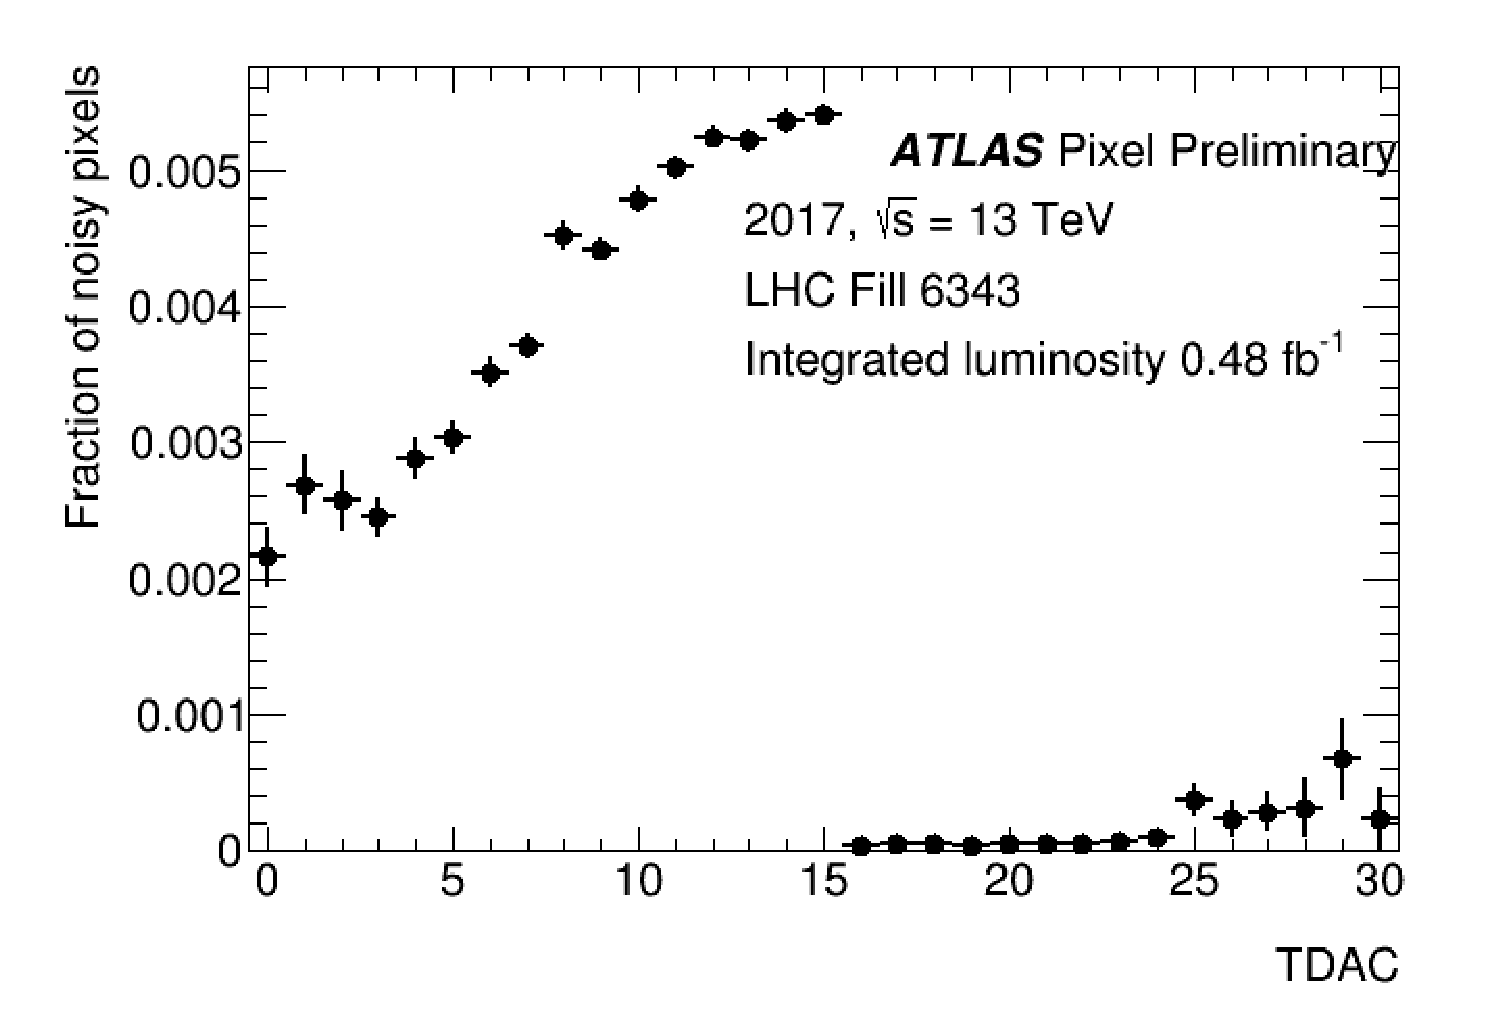
\includegraphics[width=0.5\linewidth]{figures/ElectronicsChapter/ATLAS/noiseVSTDAC_fill6343.eps}
\caption{Fraction of noisy pixels as a function of pixel TDAC during empty bunches of LHC fill 6343. TDAC values for each pixel are taken from the initial pixel configuration. The pixels with more than 200 hits in this fill are treated as noisy.}
\label{fig:noiseVSTDAC}
\end{figure}

Fig.~\ref{fig:noiseVSTDAC} shows the fraction of noisy pixels (meaning pixels that fire in correspondence with empty and well isolated bunches in the LHC ring) as a function of pixel TDAC, for a typical LHC fill in 2017. TDAC values for each pixel are taken from the initial pixel configuration. The pixels with more than 200 hits in this fill are defined as noisy. Low values of TDAC correspond to high thresholds. The higher fraction of noisy pixels with initial TDAC $< 15$ indicates that some pixels become noisy due to the SEU flip $0\rightarrow1$ of the most significant bit (MSB) of TDAC, which lowers the pixel threshold by $\sim$ 1850 e (with 2500 e being the typical discrimination threshold). No correlation of the noise with FDAC values was observed.

On the other hand, a pixel is defined to be quiet if it fired zero times in $16 pb^{-1}$ of data taking. The fraction of quiet pixels versus integrated luminosity ($\mathcal{L}$) in the 14 modules in the most forward IBL rings. The number of quiet pixels increases during data taking due to the accumulation of pixels with a flipped Enable bit. In two modules one can observe a fast drop of the number of quiet pixels due to the reconfiguration of these modules.

\begin{figure}[h]
\centering
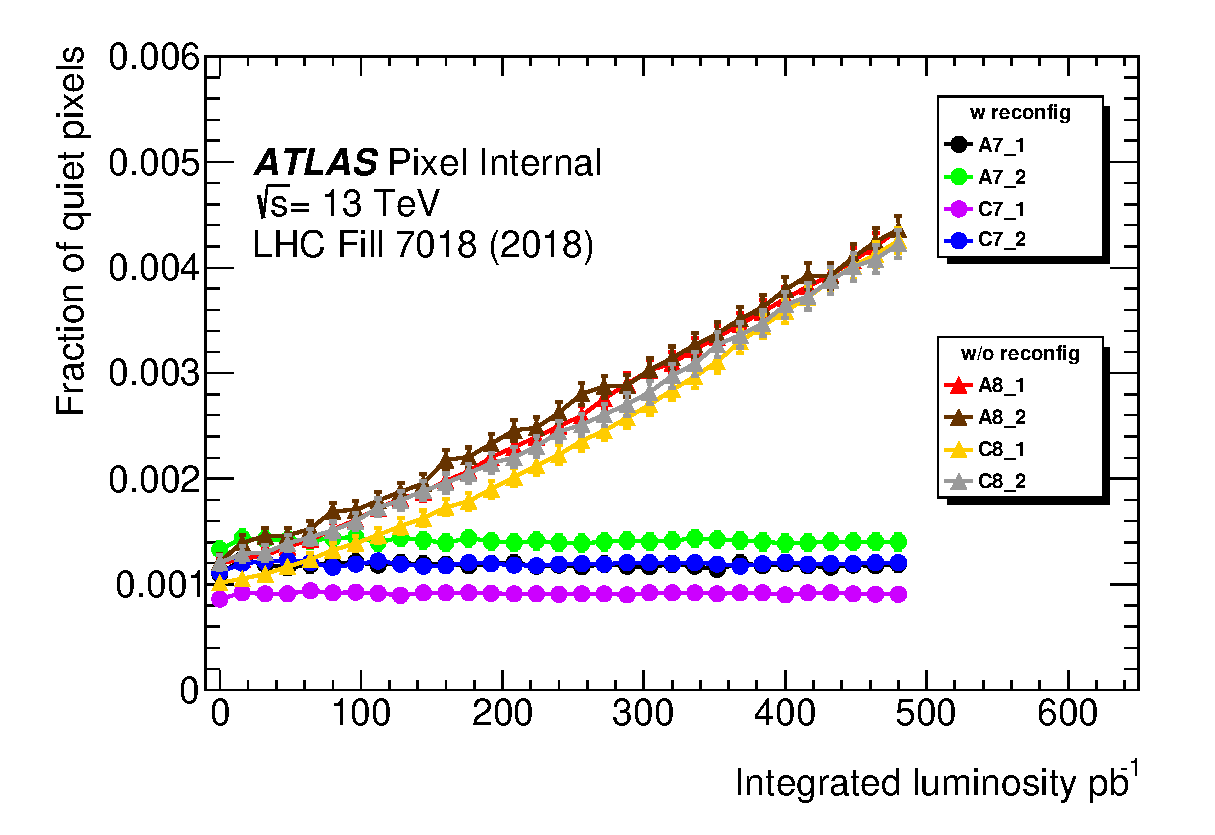
\includegraphics[width=0.49\linewidth]{figures/ElectronicsChapter/ATLAS/Quiet_357451_3D.eps}
\put(50,-5){(a)}
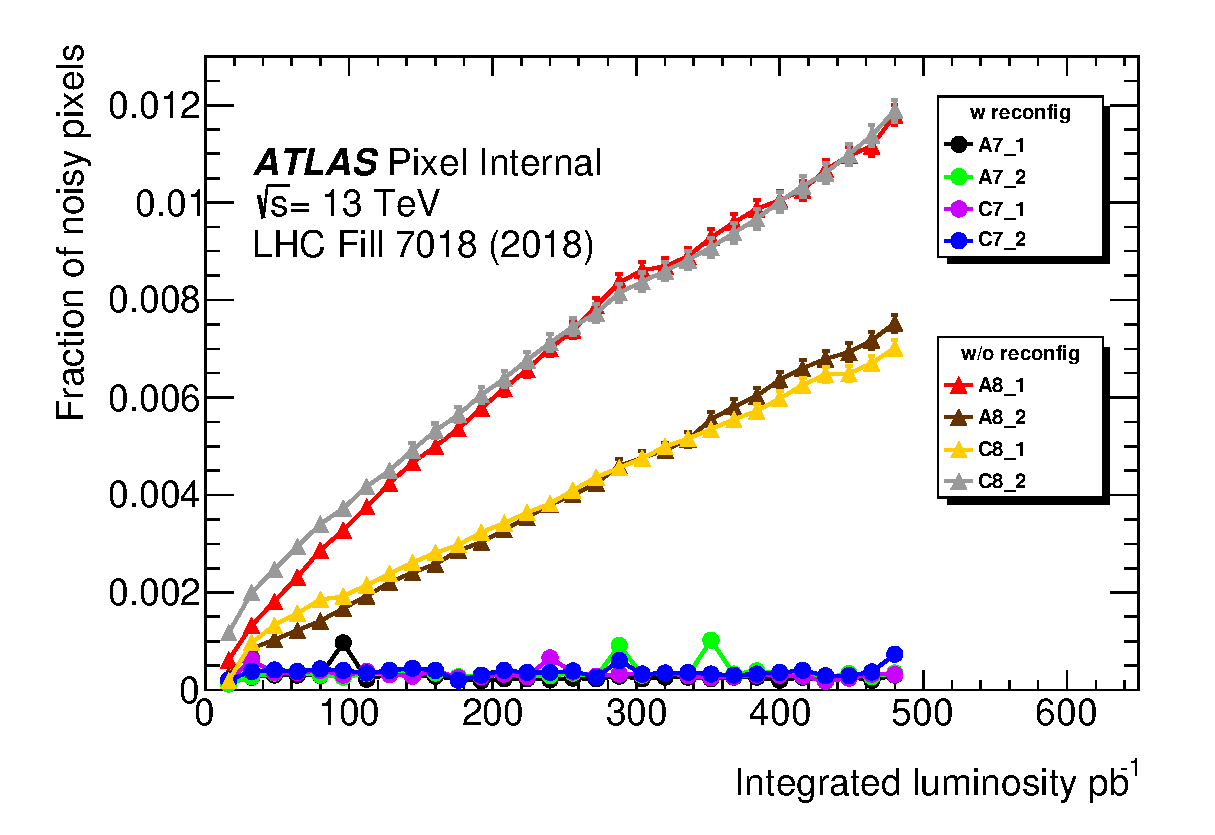
\includegraphics[width=0.49\linewidth]{figures/ElectronicsChapter/ATLAS/Noise_357451_3D.eps}
\put(50,-5){(b)}
\vspace{0.15cm}
\caption{Fraction of quiet (a) or noisy (b) pixels versus integrated luminosity in fill 7018 from 2018, shown in the eight 3D IBL $\eta$ rings.}
\label{fig:noisy-quiet-fill7018}
\end{figure}

\begin{figure}[h]
\centering
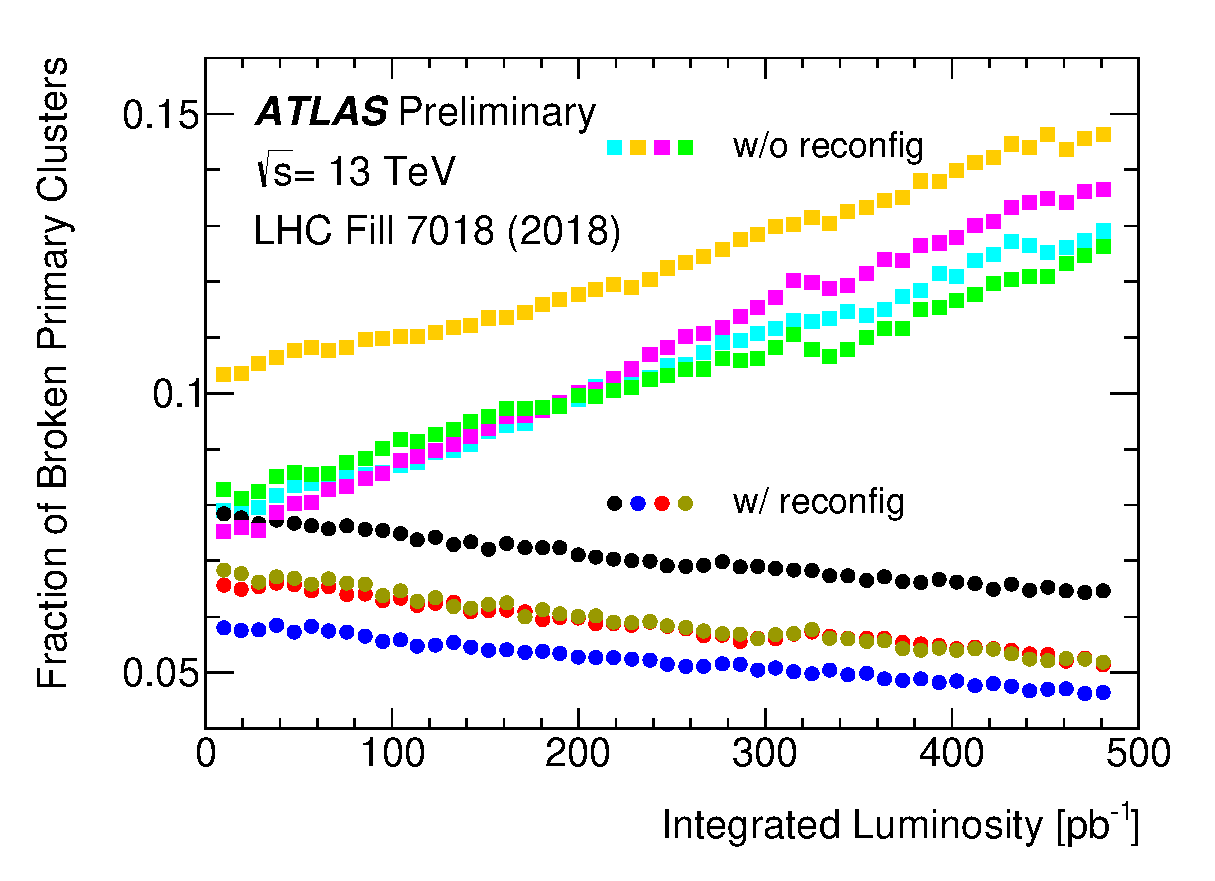
\includegraphics[width=0.49\linewidth]{figures/ElectronicsChapter/ATLAS/brokenVSlumi_run357451.eps}
\caption{Fraction of broken primary clusters versus integrated luminosity in fill 7018 from 2018, shown in the eight rings of 3D modules.}
\label{fig:broken-fill7018}
\end{figure}

Module-to-module differences in the initial number of quiet pixels indicate different fractions of silent pixels, which fire zero times during the entire fill. The fraction of pixels that become quiet due to SEU is seen to increase linearly with integrated luminosity.
 The dependence of the number of quiet pixels as the function of luminosity
was fitted with a linear function $p_0+p_1\cdot\mathcal{L}$, where the mean $p_1$ is  $5.4 \pm 1.3 \times10^{-3}$ fb.

The fraction of pixels that become quiet due to SEU ($p_1\cdot\mathcal{L}$) is equal to the ratio $\frac{N_{\textrm{errors}}}{N_{\textrm{latches}}}$ in Eq.~\ref{eq:cs-new}.  The pixel latch SEU cross section in FE-I4B is calculated with the ``quiet-pixels-fraction":
\vspace{-0.5cm}
\begin{center}
\begin{equation}
\label{eq:cs-new}
\sigma=\frac{p_1\cdot\mathcal{L}}{\Phi}
\end{equation}
\end{center}
The predicted flux of hadrons with energy above 20 MeV with PYTHIA/FLUKA simulations in the extreme outside 3D sensor IBL module
is ${\Phi}= 0.91\times10^{13}$ hadrons (T>20 MeV) cm$^{-2}$ per $1 fb^{-1}$  ~\cite{ref:IanDawson}.
 The SEU cross section is calculated to be $(0.60 \pm 0.14) \times10^{-15}$cm$^{2}$,
which is of the same order of magnitude as the test beam result.

Fig.~\ref{fig:zDep_fill5163} shows the average fraction of quiet pixels in each chip ring after $\sim$480\,pb$^{-1}$ of data taking in LHC fill 7018. It is compared with the PYTHIA/FLUKA simulation, which is normalized to the average fraction in data.

\begin{figure}[h]
\centering
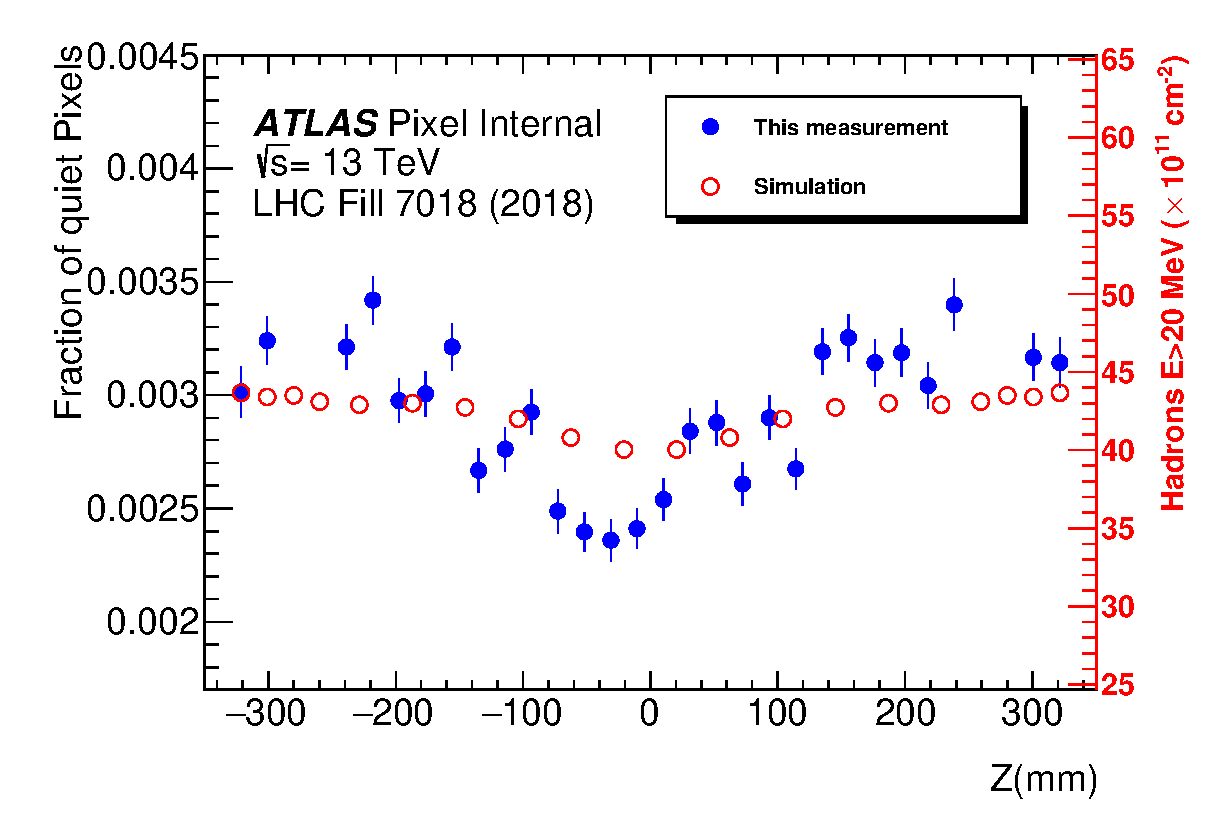
\includegraphics[width=0.49\linewidth]{figures/ElectronicsChapter/ATLAS/Fraction_357451.eps}
\vspace{0.5cm}
\caption{Average fraction of quiet pixels in each IBL chip ring after $\sim$480\,pb$^{-1}$ of data taking in LHC fill 7018 of 2018, compared with PYTHIA/FLUKA simulations. Four points are missing due to the reconfiguration tests happening during that fill in four specific front-end rings.}
\label{fig:zDep_fill5163}
\end{figure}

\begin{figure}[h]
\centering
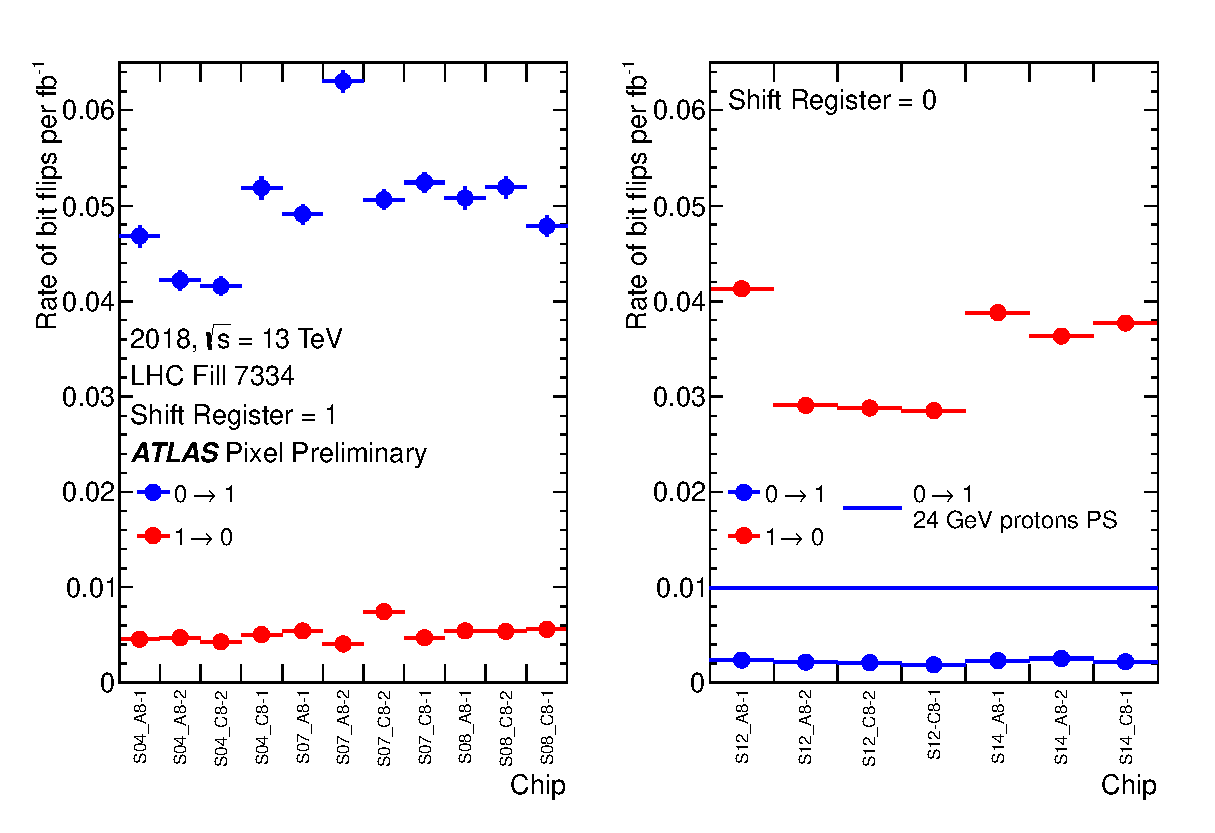
\includegraphics[width=0.9\linewidth]{figures/ElectronicsChapter/ATLAS/hrvschipsr10_line.eps}
\put(25,-1){(a)}
\put(75,-1){(b)}
\caption{
In figure (a), the Shift Register (SR) was set to 1, and $0\rightarrow1$ flips dominate due to the SET on the LOAD line, while low rate $1\rightarrow0$ flips are due to real memory SEU. In 
figure (b), the Shift Register was set to 0, and $1\rightarrow0$ flips dominate. The values of the Shift Register are refreshed several times during the fill.
The extrapolation of the measurement of SEU rate with 24 GeV protons on CERN PS is shown with blue line on the figure (b). During CERN PS measurement
the value of SR was not refreshed which may explain higher rate of bit flips due to SET contribution. 
}
\label{fig:hrvschipsr10}
\end{figure}

\begin{figure}[h]
\centering
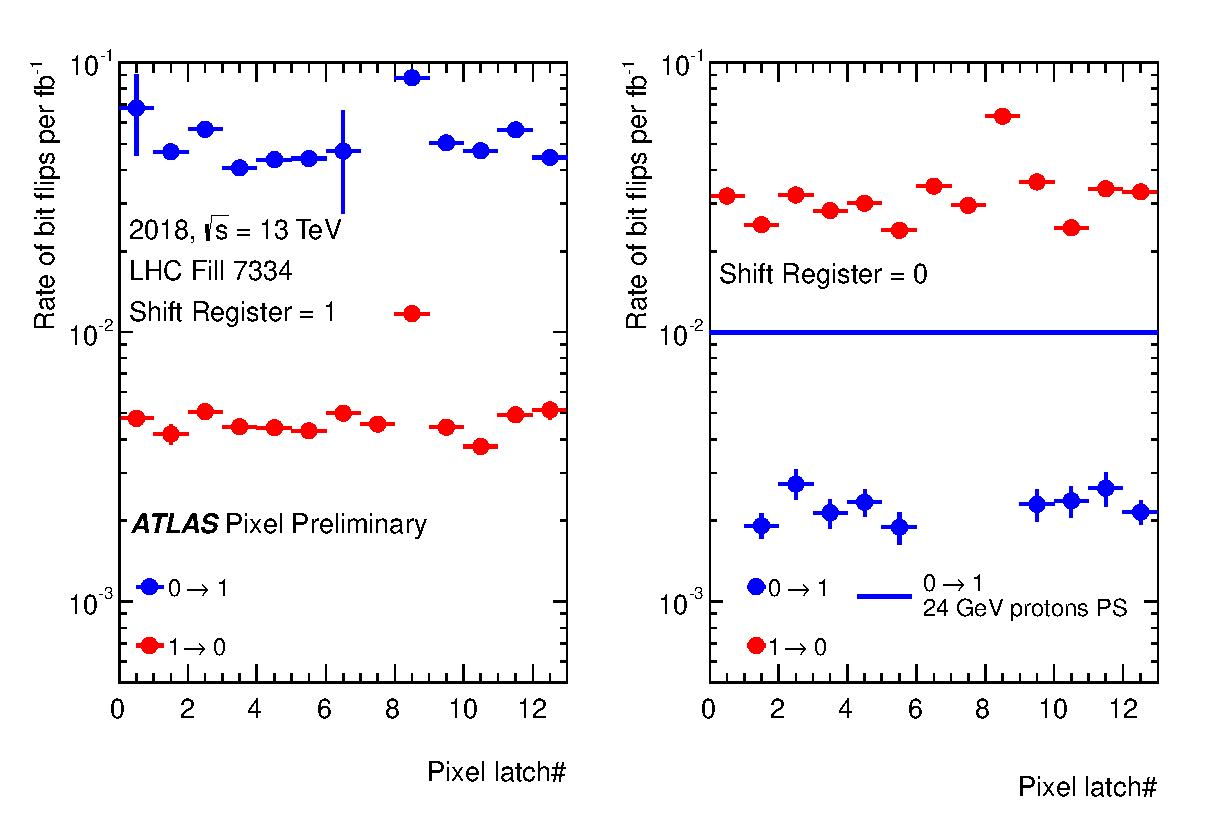
\includegraphics[width=0.9\linewidth]{figures/ElectronicsChapter/ATLAS/hrvsbitsr10_line_p.eps}
\put(25,-1){(a)}
\put(75,-1){(b)}
\caption{
Average rate of SEU/SET bit flips in pixel memory of FE-I4 per fb$^{-1}$ in LHC fill 7334, as a function of bit number (0-12). In figure (a), the Shift
Register was set to 1, and $0\rightarrow1$ flips dominate due to the glitches on the LOAD line, while low rate $1\rightarrow0$ flips are due to real memory 
SEU. In figure (b), the Shift Register was set to 0, and $1\rightarrow0$ flips dominate. The extrapolation of the measurement of the SEU rate with 24 GeV protons at CERN PS is 
shown with a blue line. During the CERN PS measurement,  the value of the SR was not refreshed, which may explain higher rate of bit flips due to SET contributions. 
}
\label{fig:hrvsbitsr10}
\end{figure}

\begin{figure}[h]
\centering
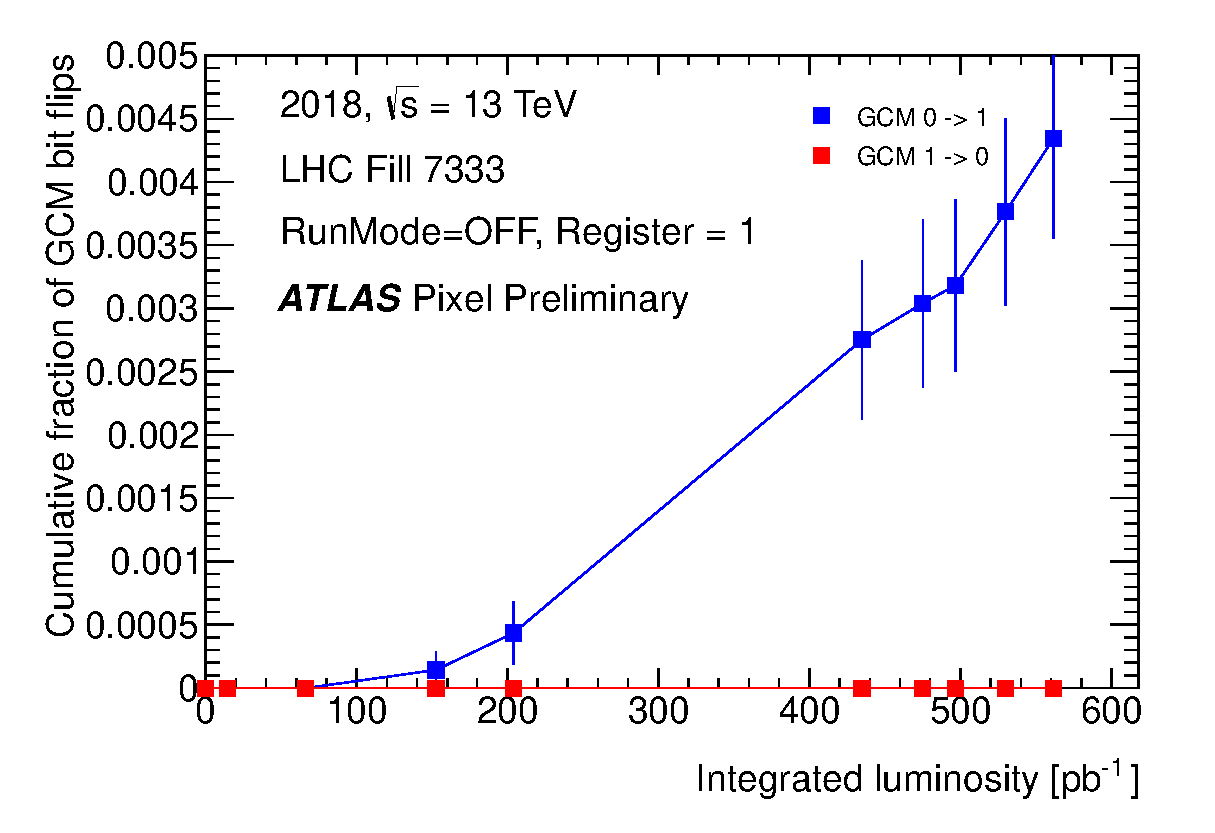
\includegraphics[width=0.49\linewidth]{figures/ElectronicsChapter/ATLAS/grseuvslumi.eps}
\caption{ Cumulative fraction of SEU/SET bit flips in the Global Configuration Memory (GCM) of FE-I4 as a function of integrated luminosity in LHC fill 7333.}
\label{fig:grseuvslumi}
\end{figure}


\subsubsubsection{SEU in SCT front-end chips (\textbf{4 pp})}

\begin{itemize}
\item SCT (\textbf{2 pp}): 
        \begin{itemize}
        \item SEU expected rate vs observed rate. Highlight the discrepancy. References to Test beam studies.
        \item Bit flip effects on de-syncronization
        \item Explanation of mitigation strategies also for SCT.
        \end{itemize}
\end{itemize}

\subsubsection{Optical links studies in SCT (\textbf{2 pp})}
\label{sec:electronics-ATLAS-Opto}
Contributing authors: T.~Weidberg, D. Robinson,

A description of radiation effects on VCSEL behaviour should go in the general part? Section 2.3?
\begin{itemize}
\item P-i-N diode: trends of the current consumption and depletion voltage estimate (test beam vs in-situ)
\item VSEL: trends of current consumption from the Off detector electronics (test beam vs in-situ)
\end{itemize}

\subsubsection{Irradiation effects in TRT electronics (2 pp)}
\label{sec:electronics-ATLAS-TRT}
Contributing author: S. Chen

\subsection{CMS}
\label{sec:electronics-CMS}

\subsection{ALICE and LHCb }
\label{sec:electronics-ALICE-LHCb}

\subsection{Inter-experiment comparisons}
\label{sec:electronics-comparisons}

\subsection{Discussion and future strategies}
\label{sec:electronics-conclusions}
Drawing conclusions from across the experiments. 


\begin{thebibliography}{99}
%ATLAS ID GENERAL from ATLAS Run1
\bibitem{jinst3s08003}
G.Aad \emph{et al.} (ATLAS Collaboration), \emph{The ATLAS Experiment at the CERN Large Hadron Collider}, \emph{JINST} {\bf 3} (2008) S08003

%ATLAS IBL Electronics
\bibitem{IBLPaper} ATLAS IBL Collaboration, Production and Integration of the ATLAS Insertable B-Layer, JINST 13 (2018) T05008.

\bibitem{FEI4} M. Garcia-Sciveres et al., The FE-I4 Pixel Readout Integrated Circuit, Nucl. Instr. and Meth A636 (2010) S155. 

\bibitem{TaskForceNote} ATLAS Collaboration, Radiation induced effects in the ATLAS Insertable B-Layer readout chip, ATL-INDET-PUB-2017-001, https://cds.cern.ch/record/2291800.

\bibitem{FACCIO} F. Faccio, G. Cervelli, Radiation-Induced Edge Effects in Deep Submicron CMOS Transistors, IEEE Trans. Nucl. Sci. 52 (2005) 2413. 

\bibitem{LAURA} L. Gonella, et al., Total Ionizing Dose effects in 130-nm commercial CMOS technologies for HEP experiments, Nucl. Instr. and Meth A582 (2007) 750.

\bibitem{MALTE} M. Backhaus, Parametrisation of the radiation induced leakage current increase of NMOS transistors,  JINST 12 (2017) P01011.

\bibitem{TWEPP2012} M. Menouni et al., SEU tolerant memory design for the ATLAS pixel readout chip, JINST 8 (2013), C02026.

\bibitem{DICE} T. Calin, M. Nicolaidis and R. Velazco, Upset hardened memory by design for submicron CMOS technology SEU, IEEE Trans. Nucl. Sci. 43 (1996) 2874.

%ATLAS SCT Electronis

%ATLAS TRT Electronics

\end{thebibliography}
